\batchmode


\documentclass{article}
\RequirePackage{ifthen}


\usepackage{html,makeidx,epsf}
\usepackage{graphicx}
\usepackage{amssymb}
\usepackage{amsmath}
\usepackage[overload]{empheq}


\htmladdtonavigation{\htmladdnormallink
  {\htmladdimg{jetscalecropped.png}}{cv.pdf}}


\makeindex




\usepackage{xcolor}

\usepackage[]{inputenc}



\makeatletter

\makeatletter
\count@=\the\catcode`\_ \catcode`\_=8 
\newenvironment{tex2html_wrap}{}{}%
\catcode`\<=12\catcode`\_=\count@
\newcommand{\providedcommand}[1]{\expandafter\providecommand\csname #1\endcsname}%
\newcommand{\renewedcommand}[1]{\expandafter\providecommand\csname #1\endcsname{}%
  \expandafter\renewcommand\csname #1\endcsname}%
\newcommand{\newedenvironment}[1]{\newenvironment{#1}{}{}\renewenvironment{#1}}%
\let\newedcommand\renewedcommand
\let\renewedenvironment\newedenvironment
\makeatother
\let\mathon=$
\let\mathoff=$
\ifx\AtBeginDocument\undefined \newcommand{\AtBeginDocument}[1]{}\fi
\newbox\sizebox
\setlength{\hoffset}{0pt}\setlength{\voffset}{0pt}
\addtolength{\textheight}{\footskip}\setlength{\footskip}{0pt}
\addtolength{\textheight}{\topmargin}\setlength{\topmargin}{0pt}
\addtolength{\textheight}{\headheight}\setlength{\headheight}{0pt}
\addtolength{\textheight}{\headsep}\setlength{\headsep}{0pt}
\setlength{\textwidth}{349pt}
\newwrite\lthtmlwrite
\makeatletter
\let\realnormalsize=\normalsize
\global\topskip=2sp
\def\preveqno{}\let\real@float=\@float \let\realend@float=\end@float
\def\@float{\let\@savefreelist\@freelist\real@float}
\def\liih@math{\ifmmode$\else\bad@math\fi}
\def\end@float{\realend@float\global\let\@freelist\@savefreelist}
\let\real@dbflt=\@dbflt \let\end@dblfloat=\end@float
\let\@largefloatcheck=\relax
\let\if@boxedmulticols=\iftrue
\def\@dbflt{\let\@savefreelist\@freelist\real@dbflt}
\def\adjustnormalsize{\def\normalsize{\mathsurround=0pt \realnormalsize
 \parindent=0pt\abovedisplayskip=0pt\belowdisplayskip=0pt}%
 \def\phantompar{\csname par\endcsname}\normalsize}%
\def\lthtmltypeout#1{{\let\protect\string \immediate\write\lthtmlwrite{#1}}}%
\usepackage[tightpage,active]{preview}
\newbox\lthtmlPageBox
\newdimen\lthtmlCropMarkHeight
\newdimen\lthtmlCropMarkDepth
\long\def\lthtmlTightVBox#1#2{%
    \setbox\lthtmlPageBox\vbox{\hbox{\catcode`\_=8 #2}}%
    \lthtmlCropMarkHeight=\ht\lthtmlPageBox \advance \lthtmlCropMarkHeight 6pt
    \lthtmlCropMarkDepth=\dp\lthtmlPageBox
    \lthtmltypeout{^^J:#1:lthtmlCropMarkHeight:=\the\lthtmlCropMarkHeight}%
    \lthtmltypeout{^^J:#1:lthtmlCropMarkDepth:=\the\lthtmlCropMarkDepth:1ex:=\the \dimexpr 1ex}%
    \begin{preview}\copy\lthtmlPageBox\end{preview}}%
\long\def\lthtmlTightFBox#1#2{%
    \adjustnormalsize\setbox\lthtmlPageBox=\vbox\bgroup %
    \let\ifinner=\iffalse \let\)\liih@math %
    {\catcode`\_=8 #2}%
    \@next\next\@currlist{}{\def\next{\voidb@x}}%
    \expandafter\box\next\egroup %
    \lthtmlCropMarkHeight=\ht\lthtmlPageBox \advance \lthtmlCropMarkHeight 6pt
    \lthtmlCropMarkDepth=\dp\lthtmlPageBox
    \lthtmltypeout{^^J:#1:lthtmlCropMarkHeight:=\the\lthtmlCropMarkHeight}%
    \lthtmltypeout{^^J:#1:lthtmlCropMarkDepth:=\the\lthtmlCropMarkDepth:1ex:=\the \dimexpr 1ex}%
    \begin{preview}\copy\lthtmlPageBox\end{preview}}%
    \long\def\lthtmlinlinemathA#1#2\lthtmlindisplaymathZ{\lthtmlTightVBox{#1}{#2}}
    \def\lthtmlinlineA#1#2\lthtmlinlineZ{\lthtmlTightVBox{#1}{#2}}
    \long\def\lthtmldisplayA#1#2\lthtmldisplayZ{\lthtmlTightVBox{#1}{#2}}
    \long\def\lthtmlinlinemathA#1#2\lthtmlindisplaymathZ{\lthtmlTightVBox{#1}{#2}}
    \def\lthtmlinlineA#1#2\lthtmlinlineZ{\lthtmlTightVBox{#1}{#2}}
    \long\def\lthtmldisplayA#1#2\lthtmldisplayZ{\lthtmlTightVBox{#1}{#2}}
    \long\def\lthtmldisplayB#1#2\lthtmldisplayZ{\\edef\preveqno{(\theequation)}%
        \lthtmlTightVBox{#1}{\let\@eqnnum\relax#2}}
    \long\def\lthtmlfigureA#1#2\lthtmlfigureZ{\let\@savefreelist\@freelist
        \lthtmlTightFBox{#1}{#2}\global\let\@freelist\@savefreelist}
    \long\def\lthtmlpictureA#1#2\lthtmlpictureZ{\let\@savefreelist\@freelist
        \lthtmlTightVBox{#1}{#2}\global\let\@freelist\@savefreelist}
\def\lthtmlcheckvsize{\ifdim\ht\sizebox<\vsize 
  \ifdim\wd\sizebox<\hsize\expandafter\hfill\fi \expandafter\vfill
  \else\expandafter\vss\fi}%
\providecommand{\selectlanguage}[1]{}%
\makeatletter \tracingstats = 1 
\providecommand{\Rho}{\textrm{R}}
\providecommand{\Chi}{\textrm{X}}
\providecommand{\omicron}{\textrm{o}}
\providecommand{\Omicron}{\textrm{O}}
\providecommand{\Kappa}{\textrm{K}}
\providecommand{\Eta}{\textrm{H}}
\providecommand{\Mu}{\textrm{M}}
\providecommand{\Beta}{\textrm{B}}
\providecommand{\Epsilon}{\textrm{E}}
\providecommand{\Iota}{\textrm{J}}
\providecommand{\Alpha}{\textrm{A}}
\providecommand{\Zeta}{\textrm{Z}}
\providecommand{\Tau}{\textrm{T}}
\providecommand{\Nu}{\textrm{N}}


\begin{document}
\pagestyle{empty}\thispagestyle{empty}\lthtmltypeout{}%
\lthtmltypeout{latex2htmlLength hsize=\the\hsize}\lthtmltypeout{}%
\lthtmltypeout{latex2htmlLength vsize=\the\vsize}\lthtmltypeout{}%
\lthtmltypeout{latex2htmlLength hoffset=\the\hoffset}\lthtmltypeout{}%
\lthtmltypeout{latex2htmlLength voffset=\the\voffset}\lthtmltypeout{}%
\lthtmltypeout{latex2htmlLength topmargin=\the\topmargin}\lthtmltypeout{}%
\lthtmltypeout{latex2htmlLength topskip=\the\topskip}\lthtmltypeout{}%
\lthtmltypeout{latex2htmlLength headheight=\the\headheight}\lthtmltypeout{}%
\lthtmltypeout{latex2htmlLength headsep=\the\headsep}\lthtmltypeout{}%
\lthtmltypeout{latex2htmlLength parskip=\the\parskip}\lthtmltypeout{}%
\lthtmltypeout{latex2htmlLength oddsidemargin=\the\oddsidemargin}\lthtmltypeout{}%
\makeatletter
\if@twoside\lthtmltypeout{latex2htmlLength evensidemargin=\the\evensidemargin}%
\else\lthtmltypeout{latex2htmlLength evensidemargin=\the\oddsidemargin}\fi%
\lthtmltypeout{}%
\makeatother
\setcounter{page}{1}
\onecolumn

% !!! IMAGES START HERE !!!

\stepcounter{section}
{\newpage\clearpage
\lthtmlinlinemathA{tex2html_wrap_inline1919}%
$\textstyle \parbox{\textwidth}{
\par
I graduated in 2009 from Munkkiniemi high school. Mathematics was a subject I had naturally thrived in -- so, after some bumps and turns,  I found myself at the University of Helsinki studying mathematics. And yeah, indeed, I love mathematics -- I love the apparent universality of it. This subject is without a doubt debatable, but, at least in some sense, I like to think that mathematical truths are universal in the truest sense of the word; they are eternal, and they are the same everywhere, regardless of the physical universe we live in. Aliens in another galaxy will end up with the same mathematical truths we do. Aliens in another universe will end up with the same mathematical truths we do. Mathematics has the power to explain what we see in our everyday life. Mathematics is not only natural science but a form of art and poetry. Mathematics is music -- music is mathematics.
\par
While studying mathematics, physics, and computer science, I took some courses on economics. That inspired me to write my bachelor's thesis on optimal control theory. I worked on the problem of how increasing public investments affects the GDP. I did not find any breakthrough, but it was an intriguing subject.
\par
I proceeded with my graduate studies studying applied mathematics. I studied subjects like partial differential equations, functional analysis, dynamical systems, and  -- the University of Helsinki's pride -- complex analysis. (My thesis advisor said that, in a moral sense, you cannot graduate from the University of Helsinki without taking some courses on Complex analysis, because a lot of the discipline has been developed at the university.) In addition, as a more ``practical'' subject, I studied some inverse problems. Summa summarum, I studied a wide range of fields in mathematics.
\par
During my graduate studies, I spent half a year in Utrecht, Netherlands, studying more applied analysis of varying subjects (searching periodic orbits in the Lorentz attractor as an example of a course -- that I failed). At Utrecht University, I got the inspiration for the subject for my future master's thesis; the Finite Element Method. After I got back to Helsinki from the exchange, I had a chance to study more about the finite element method in Aalto University's courses. (Aalto University is a consortium of the Helsinki University of Technology, the Helsinki School of Economics, and the University of Art and Design Helsinki.) While writing my thesis I also taught basic mathematics courses at the University of Helsinki and gained valuable experience in the pedagogical area.
\par
In the binge of graduation, I started to look for future opportunities. I looked for coding jobs in Helsinki and Tallinn, jobs for mathematicians in the mapping industry, continuing at some universities to pursue a Ph.D., etc. I am glad I had the chance to use my creativity and continue in Aalto University's Department of Signal Processing and Acoustics to research low earth orbit satellite communications. The research methodology was from a stochastic geometry perspective, which was well aligned with my mathematical background.
\par
My professional ambitions are in improving the lives of people globally. Communications play an essential in the picture. (But contain some challenging problems also, as we have seen with social media.) Through effective communication, we can share knowledge, control resources, discuss issues, etc. -- however, globally, the communication infrastructure is still not nearly complete. My interests contain, but are not limited to, communications, particularly wireless networks and signal processing. My dream is to share my knowledge in the process toward a free and honest world. (Pardon me for the cliches.)
\par
}$%
\lthtmlindisplaymathZ
\lthtmlcheckvsize\clearpage}

\stepcounter{subsection}
\stepcounter{subsection}
\stepcounter{subsection}
\stepcounter{subsection}
\stepcounter{section}
\stepcounter{subsection}
{\newpage\clearpage
\lthtmlinlinemathA{tex2html_wrap_inline1930}%
$ A = [-\pi,\pi] \times [-1,1]$%
\lthtmlindisplaymathZ
\lthtmlcheckvsize\clearpage}

{\newpage\clearpage
\lthtmlinlinemathA{tex2html_wrap_inline1932}%
$ A$%
\lthtmlindisplaymathZ
\lthtmlcheckvsize\clearpage}

{\newpage\clearpage
\lthtmlinlinemathA{tex2html_wrap_indisplay1934}%
$\displaystyle (x,y) \mapsto (1,x,\sin^{-1}(y)) .$%
\lthtmlindisplaymathZ
\lthtmlcheckvsize\clearpage}

{\newpage\clearpage
\lthtmlinlinemathA{tex2html_wrap_inline1936}%
$ (r,\theta,\varphi)$%
\lthtmlindisplaymathZ
\lthtmlcheckvsize\clearpage}

{\newpage\clearpage
\lthtmlinlinemathA{tex2html_wrap_inline1938}%
$ r$%
\lthtmlindisplaymathZ
\lthtmlcheckvsize\clearpage}

\stepcounter{subsection}
\stepcounter{subsection}
\stepcounter{subsection}
\stepcounter{subsection}
\stepcounter{subsection}
{\newpage\clearpage
\lthtmlinlinemathA{tex2html_wrap_inline1962}%
$ B$%
\lthtmlindisplaymathZ
\lthtmlcheckvsize\clearpage}

{\newpage\clearpage
\lthtmlinlinemathA{tex2html_wrap_indisplay1964}%
$\displaystyle \textbf{P}[$%
\lthtmlindisplaymathZ
\lthtmlcheckvsize\clearpage}

{\newpage\clearpage
\lthtmlinlinemathA{tex2html_wrap_indisplay1965}%
$\displaystyle ] = e^{-\frac{\pi^2}{2\sqrt{P}}},$%
\lthtmlindisplaymathZ
\lthtmlcheckvsize\clearpage}

{\newpage\clearpage
\lthtmlinlinemathA{tex2html_wrap_inline1967}%
$ P$%
\lthtmlindisplaymathZ
\lthtmlcheckvsize\clearpage}

{\newpage\clearpage
\lthtmlinlinemathA{tex2html_wrap_inline1969}%
$ (1)$%
\lthtmlindisplaymathZ
\lthtmlcheckvsize\clearpage}

{\newpage\clearpage
\lthtmlinlinemathA{tex2html_wrap_indisplay1972}%
$\displaystyle ]  = 1-\left(1-e^{-\frac{\pi^2}{2\sqrt{P/N}}}\right)^N,$%
\lthtmlindisplaymathZ
\lthtmlcheckvsize\clearpage}

{\newpage\clearpage
\lthtmlinlinemathA{tex2html_wrap_inline1974}%
$ N$%
\lthtmlindisplaymathZ
\lthtmlcheckvsize\clearpage}

\stepcounter{subsection}
\stepcounter{subsection}
\stepcounter{subsection}
{\newpage\clearpage
\lthtmlinlinemathA{tex2html_wrap_inline1995}%
$ [0, \infty)$%
\lthtmlindisplaymathZ
\lthtmlcheckvsize\clearpage}

{\newpage\clearpage
\lthtmlinlinemathA{tex2html_wrap_inline1997}%
$ Y_j$%
\lthtmlindisplaymathZ
\lthtmlcheckvsize\clearpage}

{\newpage\clearpage
\lthtmlinlinemathA{tex2html_wrap_inline1999}%
$ B(r_1,r_2)$%
\lthtmlindisplaymathZ
\lthtmlcheckvsize\clearpage}

{\newpage\clearpage
\lthtmlinlinemathA{tex2html_wrap_inline2001}%
$ 2\int_{r_1}^{r^2} \frac{1}{\sqrt{2 \pi}}e^{-y^2} dy.$%
\lthtmlindisplaymathZ
\lthtmlcheckvsize\clearpage}

{\newpage\clearpage
\lthtmlinlinemathA{tex2html_wrap_indisplay2002}%
$\displaystyle \mathcal{L}_{\tau}(f)$%
\lthtmlindisplaymathZ
\lthtmlcheckvsize\clearpage}

{\newpage\clearpage
\lthtmlinlinemathA{tex2html_wrap_indisplay2003}%
$\displaystyle = \mathbb{E} \exp \left[-\sum_i f(|Y_i|) \right] = \mathbb{E}  \prod_i \exp \left[  -f(|Y_i|)   \right]$%
\lthtmlindisplaymathZ
\lthtmlcheckvsize\clearpage}

{\newpage\clearpage
\lthtmlinlinemathA{tex2html_wrap_indisplay2004}%
$\displaystyle = \mathbb{E}_n \left[  (2 \pi)^{-n/2}  \int_0^{\infty} \dots \int_0^{\infty}  \prod_{i = 0}^n \exp \left[  -f(y_i)  \right] \frac{2}{\sqrt{2 \pi}}e^{-y_i^2} dy_1 \dots d y_n \right]$%
\lthtmlindisplaymathZ
\lthtmlcheckvsize\clearpage}

{\newpage\clearpage
\lthtmlinlinemathA{tex2html_wrap_indisplay2005}%
$\displaystyle = \mathbb{E}_n \left[(2 \pi)^{-n/2}  \left( \int_{0}^{\infty}  2\exp \left[  -f(y) - y^2   \right] dy \right)^n\right]$%
\lthtmlindisplaymathZ
\lthtmlcheckvsize\clearpage}

{\newpage\clearpage
\lthtmlinlinemathA{tex2html_wrap_indisplay2006}%
$\displaystyle = \mathbb{E}_n \exp \left[ \sum_{i= 0}^n \log \left(   \int_{0}^{\infty}  \exp \left[  -f(y)  \right] \frac{2e^{-y^2}}{\sqrt{2 \pi}} dy \right) \right]$%
\lthtmlindisplaymathZ
\lthtmlcheckvsize\clearpage}

{\newpage\clearpage
\lthtmlinlinemathA{tex2html_wrap_inline2008}%
$ \mathcal{L}(g)$%
\lthtmlindisplaymathZ
\lthtmlcheckvsize\clearpage}

{\newpage\clearpage
\lthtmlinlinemathA{tex2html_wrap_inline2010}%
$ g = - \log \left(   \int_{0}^{\infty}  \exp \left[  -f(y)  \right] \frac{e^{-y^2}}{\sqrt{2 \pi}} dy \right)  $%
\lthtmlindisplaymathZ
\lthtmlcheckvsize\clearpage}

{\newpage\clearpage
\lthtmlinlinemathA{tex2html_wrap_indisplay2011}%
$\displaystyle \mathcal{L}(g) = \mathcal{L}_{\tau}(f)$%
\lthtmlindisplaymathZ
\lthtmlcheckvsize\clearpage}

{\newpage\clearpage
\lthtmlinlinemathA{tex2html_wrap_indisplay2012}%
$\displaystyle = \exp \left[  -\int_{\mathbb{R}^2} 1 -  e^{\log \left(   \int_{0}^{\infty}  \exp \left[  -f(y)   \right] \frac{2e^{-y^2}}{\sqrt{2 \pi}} dy \right) }\Lambda(dx) \right]$%
\lthtmlindisplaymathZ
\lthtmlcheckvsize\clearpage}

{\newpage\clearpage
\lthtmlinlinemathA{tex2html_wrap_indisplay2013}%
$\displaystyle = \exp \left[-\int_{\mathbb{R}^2} \left(1  -   \int_{0}^{\infty}  \exp [-f(y)] \frac{2e^{-y^2}}{\sqrt{2 \pi}}  dy \right)  \Lambda(dx)  \right]$%
\lthtmlindisplaymathZ
\lthtmlcheckvsize\clearpage}

{\newpage\clearpage
\lthtmlinlinemathA{tex2html_wrap_indisplay2014}%
$\displaystyle = \exp \left[-\int_{\mathbb{R}^2}\int_{0}^{\infty} \left(1  -     \exp [-f(y)]   \right) \frac{2e^{-y^2}}{\sqrt{2 \pi}}dy  \Lambda(dx)  \right]$%
\lthtmlindisplaymathZ
\lthtmlcheckvsize\clearpage}

{\newpage\clearpage
\lthtmlinlinemathA{tex2html_wrap_indisplay2015}%
$\displaystyle = \exp \left[-\int_{0}^{\infty} \left(1  -     \exp [-f(y)]   \right)  \sqrt{\frac{2}{\pi}}e^{-y^2} N dy    \right], (1)$%
\lthtmlindisplaymathZ
\lthtmlcheckvsize\clearpage}

{\newpage\clearpage
\lthtmlinlinemathA{tex2html_wrap_inline2023}%
$ \sqrt{\frac{2}{\pi}}e^{-x^2} N.$%
\lthtmlindisplaymathZ
\lthtmlcheckvsize\clearpage}

{\newpage\clearpage
\lthtmlinlinemathA{tex2html_wrap_inline2027}%
$ 10000$%
\lthtmlindisplaymathZ
\lthtmlcheckvsize\clearpage}

{\newpage\clearpage
\lthtmlpictureA{tex2html_wrap2031}%
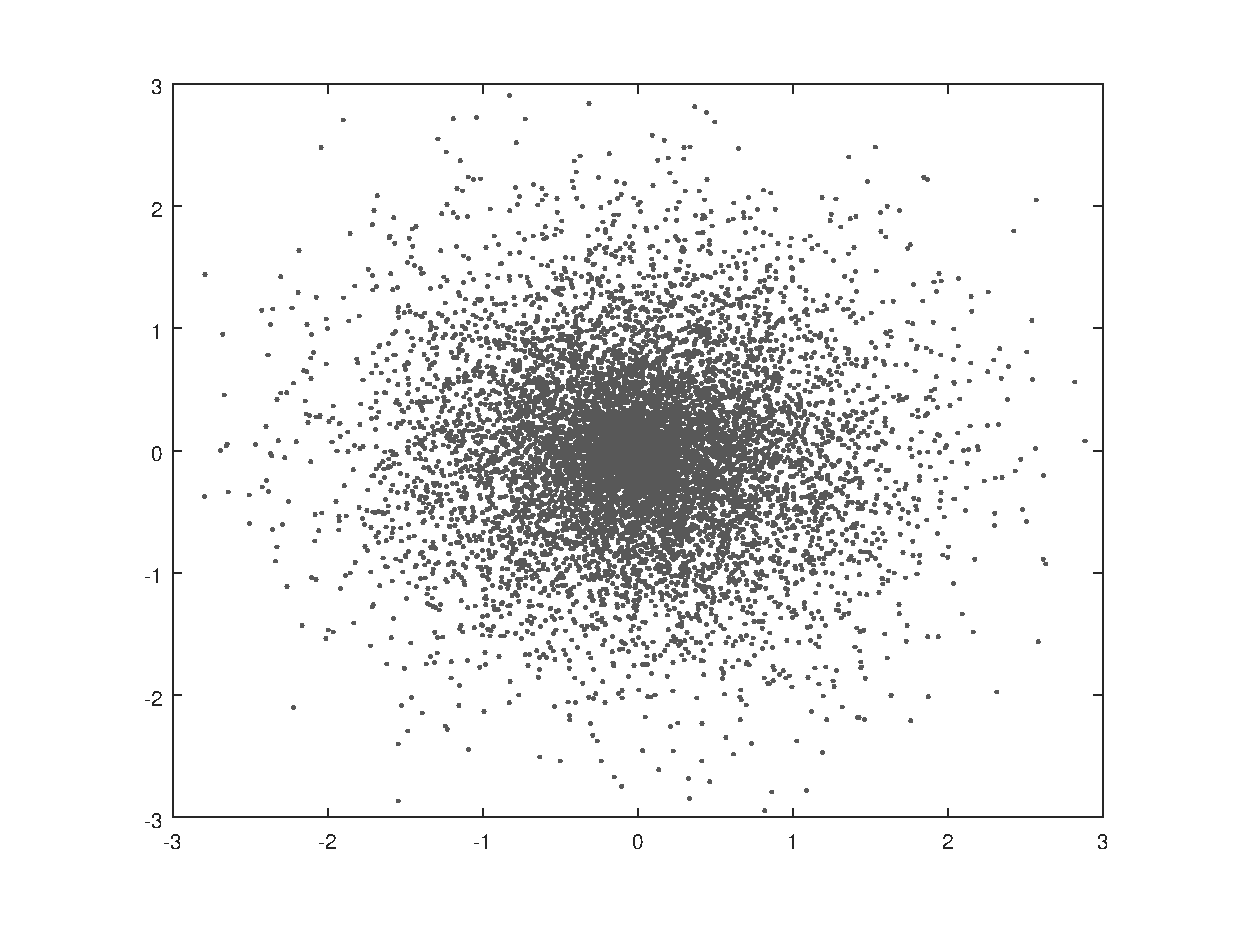
\includegraphics[width=\linewidth]{spread.eps}%
\lthtmlpictureZ
\lthtmlcheckvsize\clearpage}

\stepcounter{subsection}
{\newpage\clearpage
\lthtmlinlinemathA{tex2html_wrap_inline2034}%
$ F_s$%
\lthtmlindisplaymathZ
\lthtmlcheckvsize\clearpage}

{\newpage\clearpage
\lthtmlinlinemathA{tex2html_wrap_inline2036}%
$ F_s/2$%
\lthtmlindisplaymathZ
\lthtmlcheckvsize\clearpage}

\stepcounter{subsection}
{\newpage\clearpage
\lthtmlinlinemathA{tex2html_wrap_inline2039}%
$ S(t)$%
\lthtmlindisplaymathZ
\lthtmlcheckvsize\clearpage}

{\newpage\clearpage
\lthtmlinlinemathA{tex2html_wrap_inline2041}%
$ t \mapsto \frac{\sin(2 \pi B_L t)}{\pi t}$%
\lthtmlindisplaymathZ
\lthtmlcheckvsize\clearpage}

{\newpage\clearpage
\lthtmlinlinemathA{tex2html_wrap_inline2045}%
$ B_L$%
\lthtmlindisplaymathZ
\lthtmlcheckvsize\clearpage}

{\newpage\clearpage
\lthtmlinlinemathA{tex2html_wrap_inline2047}%
$ t \mapsto \delta(t) -  \frac{\sin(2 \pi B_H t)}{\pi t},$%
\lthtmlindisplaymathZ
\lthtmlcheckvsize\clearpage}

{\newpage\clearpage
\lthtmlinlinemathA{tex2html_wrap_inline2049}%
$ \delta(t)$%
\lthtmlindisplaymathZ
\lthtmlcheckvsize\clearpage}

{\newpage\clearpage
\lthtmlinlinemathA{tex2html_wrap_inline2051}%
$ B_H$%
\lthtmlindisplaymathZ
\lthtmlcheckvsize\clearpage}

{\newpage\clearpage
\lthtmlinlinemathA{tex2html_wrap_indisplay2053}%
$\displaystyle \mathbb{Z} \ni i \mapsto \frac{\sin(2 \pi \frac{B_L}{f_c} i)}{\pi i},
$%
\lthtmlindisplaymathZ
\lthtmlcheckvsize\clearpage}

{\newpage\clearpage
\lthtmlinlinemathA{tex2html_wrap_indisplay2055}%
$\displaystyle i \mapsto \delta[i] - \frac{\sin(2 \pi \frac{B_H}{f_c} i)}{\pi i},
$%
\lthtmlindisplaymathZ
\lthtmlcheckvsize\clearpage}

{\newpage\clearpage
\lthtmlinlinemathA{tex2html_wrap_inline2057}%
$ f_c$%
\lthtmlindisplaymathZ
\lthtmlcheckvsize\clearpage}

{\newpage\clearpage
\lthtmlinlinemathA{tex2html_wrap_inline2059}%
$ i \mapsto \delta[i] := \delta_{0i} $%
\lthtmlindisplaymathZ
\lthtmlcheckvsize\clearpage}

{\newpage\clearpage
\lthtmlinlinemathA{tex2html_wrap_inline2063}%
$ \cos(20 \pi t) + \sin(2 \pi t)$%
\lthtmlindisplaymathZ
\lthtmlcheckvsize\clearpage}

\stepcounter{subsection}
{\newpage\clearpage
\lthtmlinlinemathA{tex2html_wrap_inline2072}%
$ (-2,10) \times(-10i, 10i) \subset \mathbb{C}.$%
\lthtmlindisplaymathZ
\lthtmlcheckvsize\clearpage}

{\newpage\clearpage
\lthtmlinlinemathA{tex2html_wrap_inline2074}%
$ \max = 2$%
\lthtmlindisplaymathZ
\lthtmlcheckvsize\clearpage}

{\newpage\clearpage
\lthtmlinlinemathA{tex2html_wrap_inline2078}%
$ 0.1$%
\lthtmlindisplaymathZ
\lthtmlcheckvsize\clearpage}

\stepcounter{section}
\stepcounter{subsection}
{\newpage\clearpage
\lthtmlinlinemathA{tex2html_wrap_inline2082}%
$ X \sim \mathcal{N}(\mu, \sigma^2)$%
\lthtmlindisplaymathZ
\lthtmlcheckvsize\clearpage}

{\newpage\clearpage
\lthtmlinlinemathA{tex2html_wrap_inline2084}%
$ X \approx Y \sim$%
\lthtmlindisplaymathZ
\lthtmlcheckvsize\clearpage}

{\newpage\clearpage
\lthtmlinlinemathA{tex2html_wrap_inline2085}%
$ (\mu_{\text{LN}}, \sigma_{\text{LN}}),$%
\lthtmlindisplaymathZ
\lthtmlcheckvsize\clearpage}

{\newpage\clearpage
\lthtmlinlinemathA{tex2html_wrap_indisplay2087}%
$\displaystyle \mu = \exp\left( \mu_{\text{LN}} + \frac{\sigma_{\text{LN}}^2}{2} \right)$%
\lthtmlindisplaymathZ
\lthtmlcheckvsize\clearpage}

{\newpage\clearpage
\lthtmlinlinemathA{tex2html_wrap_indisplay2089}%
$\displaystyle \sigma = (\exp( \sigma_{\text{LN}}^2) - 1)\exp(2 \mu_{\text{LN}} + \sigma_{\text{LN}}^2).$%
\lthtmlindisplaymathZ
\lthtmlcheckvsize\clearpage}

{\newpage\clearpage
\lthtmlinlinemathA{tex2html_wrap_inline2091}%
$ \mu_{\text{LN}}$%
\lthtmlindisplaymathZ
\lthtmlcheckvsize\clearpage}

{\newpage\clearpage
\lthtmlinlinemathA{tex2html_wrap_inline2093}%
$ \sigma_{\text{LN}}$%
\lthtmlindisplaymathZ
\lthtmlcheckvsize\clearpage}

{\newpage\clearpage
\lthtmlinlinemathA{tex2html_wrap_inline2095}%
$ X$%
\lthtmlindisplaymathZ
\lthtmlcheckvsize\clearpage}

{\newpage\clearpage
\lthtmlinlinemathA{tex2html_wrap_indisplay2097}%
$\displaystyle 1/X \approx 1/Y \sim$%
\lthtmlindisplaymathZ
\lthtmlcheckvsize\clearpage}

{\newpage\clearpage
\lthtmlinlinemathA{tex2html_wrap_indisplay2098}%
$\displaystyle (-\mu_{\text{LN}}, \sigma_{\text{LN}}).
$%
\lthtmlindisplaymathZ
\lthtmlcheckvsize\clearpage}

\stepcounter{subsection}
\stepcounter{subsection}
\stepcounter{subsection}
{\newpage\clearpage
\lthtmlinlinemathA{tex2html_wrap_inline2103}%
$ 2000$%
\lthtmlindisplaymathZ
\lthtmlcheckvsize\clearpage}

{\newpage\clearpage
\lthtmlinlinemathA{tex2html_wrap_inline2105}%
$ 35$%
\lthtmlindisplaymathZ
\lthtmlcheckvsize\clearpage}

{\newpage\clearpage
\lthtmlinlinemathA{tex2html_wrap_inline2107}%
$ 3$%
\lthtmlindisplaymathZ
\lthtmlcheckvsize\clearpage}

{\newpage\clearpage
\lthtmlinlinemathA{tex2html_wrap_inline2109}%
$ 1.5$%
\lthtmlindisplaymathZ
\lthtmlcheckvsize\clearpage}

\stepcounter{subsection}
{\newpage\clearpage
\lthtmlinlinemathA{tex2html_wrap_inline2112}%
$ t$%
\lthtmlindisplaymathZ
\lthtmlcheckvsize\clearpage}

{\newpage\clearpage
\lthtmlinlinemathA{tex2html_wrap_indisplay2114}%
$\displaystyle \{t \mapsto$%
\lthtmlindisplaymathZ
\lthtmlcheckvsize\clearpage}

{\newpage\clearpage
\lthtmlinlinemathA{tex2html_wrap_indisplay2115}%
$\displaystyle (F_s t - n)\}_n,
$%
\lthtmlindisplaymathZ
\lthtmlcheckvsize\clearpage}

{\newpage\clearpage
\lthtmlinlinemathA{tex2html_wrap_indisplay2121}%
$\displaystyle \{ x[n]\}_{n=0}^{N-1}
$%
\lthtmlindisplaymathZ
\lthtmlcheckvsize\clearpage}

{\newpage\clearpage
\lthtmlinlinemathA{tex2html_wrap_indisplay2123}%
$\displaystyle S(t) =\sum_{n = 0}^{N-1} x[n]$%
\lthtmlindisplaymathZ
\lthtmlcheckvsize\clearpage}

{\newpage\clearpage
\lthtmlinlinemathA{tex2html_wrap_indisplay2124}%
$\displaystyle (F_s t - n),
$%
\lthtmlindisplaymathZ
\lthtmlcheckvsize\clearpage}

{\newpage\clearpage
\lthtmlinlinemathA{tex2html_wrap_inline2128}%
$ x$%
\lthtmlindisplaymathZ
\lthtmlcheckvsize\clearpage}

{\newpage\clearpage
\lthtmlinlinemathA{tex2html_wrap_inline2130}%
$ S$%
\lthtmlindisplaymathZ
\lthtmlcheckvsize\clearpage}

\stepcounter{subsection}
{\newpage\clearpage
\lthtmlinlinemathA{tex2html_wrap_inline2137}%
$ \alpha$%
\lthtmlindisplaymathZ
\lthtmlcheckvsize\clearpage}

{\newpage\clearpage
\lthtmlinlinemathA{tex2html_wrap_inline2141}%
$ \alpha = 2$%
\lthtmlindisplaymathZ
\lthtmlcheckvsize\clearpage}

{\newpage\clearpage
\lthtmlinlinemathA{tex2html_wrap_inline2143}%
$ \alpha \leq 1$%
\lthtmlindisplaymathZ
\lthtmlcheckvsize\clearpage}

{\newpage\clearpage
\lthtmlinlinemathA{tex2html_wrap_inline2149}%
$ \alpha =1$%
\lthtmlindisplaymathZ
\lthtmlcheckvsize\clearpage}

\stepcounter{subsection}
{\newpage\clearpage
\lthtmlinlinemathA{tex2html_wrap_inline2156}%
$ t \in [0,1]$%
\lthtmlindisplaymathZ
\lthtmlcheckvsize\clearpage}

{\newpage\clearpage
\lthtmlinlinemathA{tex2html_wrap_inline2158}%
$ S_1(t) = \cos(2 \pi t)$%
\lthtmlindisplaymathZ
\lthtmlcheckvsize\clearpage}

{\newpage\clearpage
\lthtmlinlinemathA{tex2html_wrap_inline2160}%
$ S_2(t) = \cos(2 \pi t + \pi).$%
\lthtmlindisplaymathZ
\lthtmlcheckvsize\clearpage}

{\newpage\clearpage
\lthtmlinlinemathA{tex2html_wrap_inline2162}%
$ S_1 + S_2$%
\lthtmlindisplaymathZ
\lthtmlcheckvsize\clearpage}

{\newpage\clearpage
\lthtmlinlinemathA{tex2html_wrap_indisplay2164}%
$\displaystyle \mathbb{E}[(S_1 + S_2)^2] = \int_0^1 (\cos(2 \pi t) + \cos(2 \pi t + \pi))^2dt = \int_0^10 dt = 0,$%
\lthtmlindisplaymathZ
\lthtmlcheckvsize\clearpage}

{\newpage\clearpage
\lthtmlinlinemathA{tex2html_wrap_inline2166}%
$ \mathbb{E}[\cdot]$%
\lthtmlindisplaymathZ
\lthtmlcheckvsize\clearpage}

{\newpage\clearpage
\lthtmlinlinemathA{tex2html_wrap_indisplay2167}%
$\displaystyle \mathbb{E}[S_1^2] + \mathbb{E}[S_2^2]$%
\lthtmlindisplaymathZ
\lthtmlcheckvsize\clearpage}

{\newpage\clearpage
\lthtmlinlinemathA{tex2html_wrap_indisplay2168}%
$\displaystyle =   \int_0^1 \cos^2(2 \pi t) dt + \int_0^1 \cos^2(2 \pi  t + \pi) dt$%
\lthtmlindisplaymathZ
\lthtmlcheckvsize\clearpage}

{\newpage\clearpage
\lthtmlinlinemathA{tex2html_wrap_indisplay2169}%
$\displaystyle = \int_0^1 2 \cos^2(2 \pi t)  dt= \int_0^1 \cos(4 \pi t)dt + 1 = 1,$%
\lthtmlindisplaymathZ
\lthtmlcheckvsize\clearpage}

{\newpage\clearpage
\lthtmlinlinemathA{tex2html_wrap_inline2171}%
$ (2)$%
\lthtmlindisplaymathZ
\lthtmlcheckvsize\clearpage}

{\newpage\clearpage
\lthtmlinlinemathA{tex2html_wrap_inline2173}%
$ S_1$%
\lthtmlindisplaymathZ
\lthtmlcheckvsize\clearpage}

{\newpage\clearpage
\lthtmlinlinemathA{tex2html_wrap_inline2175}%
$ S_2$%
\lthtmlindisplaymathZ
\lthtmlcheckvsize\clearpage}

{\newpage\clearpage
\lthtmlinlinemathA{tex2html_wrap_indisplay2177}%
$\displaystyle \mathbb{E}[(S_1 + S_2)^2] = \mathbb{E}[S_1^2 + S_2^2 + 2 S_1 S_2]= \mathbb{E}[S_1^2] + \mathbb{E}[S_2^2] + 2 \mathbb{E}[S_1 S_2],$%
\lthtmlindisplaymathZ
\lthtmlcheckvsize\clearpage}

{\newpage\clearpage
\lthtmlinlinemathA{tex2html_wrap_inline2179}%
$ \mathbb{E}[(S_1 + S_2)^2] = \mathbb{E}[S_1^2] + \mathbb{E}[S_2^2] $%
\lthtmlindisplaymathZ
\lthtmlcheckvsize\clearpage}

{\newpage\clearpage
\lthtmlinlinemathA{tex2html_wrap_inline2181}%
$ \mathbb{E}[S_1 S_2] = 0,$%
\lthtmlindisplaymathZ
\lthtmlcheckvsize\clearpage}

{\newpage\clearpage
\lthtmlinlinemathA{tex2html_wrap_indisplay2187}%
$\displaystyle \mathbb{E}[S_1S_2] = \int_0^1 \cos(2 \pi t) \cos(2 \pi t + \pi) dt =\int_0^1 -\cos^2(2 \pi t )dt = - \frac{1}{2}\int_0^1 \cos(4 \pi t)dt - \frac{1}{2} = - \frac{1}{2},
$%
\lthtmlindisplaymathZ
\lthtmlcheckvsize\clearpage}

{\newpage\clearpage
\lthtmlinlinemathA{tex2html_wrap_inline2189}%
$ \phi_1,\phi_2 \in [0,2 \pi]$%
\lthtmlindisplaymathZ
\lthtmlcheckvsize\clearpage}

{\newpage\clearpage
\lthtmlinlinemathA{tex2html_wrap_inline2191}%
$ S_1(t) = \cps(2 \pi t + \phi_1)$%
\lthtmlindisplaymathZ
\lthtmlcheckvsize\clearpage}

{\newpage\clearpage
\lthtmlinlinemathA{tex2html_wrap_inline2193}%
$ S_2(t) = \cos(2 \pi t + \phi_2)$%
\lthtmlindisplaymathZ
\lthtmlcheckvsize\clearpage}

{\newpage\clearpage
\lthtmlinlinemathA{tex2html_wrap_indisplay2194}%
$\displaystyle \mathbb{E}_{\phi_1,\phi_2} \left[\mathbb{E}[(S_1 + S_2)^2]\right] = \mathbb{E}_{\phi_1} \left[\mathbb{E}\left[ S_1^2\right]\right] + \mathbb{E}_{\phi_2} \left[\mathbb{E}\left[ S_2^2\right]\right] +\mathbb{E}_{\phi_1,\phi_2} \left[\mathbb{E}\left[ S_1S_2\right]\right]$%
\lthtmlindisplaymathZ
\lthtmlcheckvsize\clearpage}

{\newpage\clearpage
\lthtmlinlinemathA{tex2html_wrap_indisplay2195}%
$\displaystyle =\frac{1}{2 \pi}\int_0^{2 \pi} \int_0^1 (\cos(2 \pi t + \phi_1))^2dt d \phi_1 + \frac{1}{2 \pi}\int_0^{2 \pi} \int_0^1 ( \cos(2 \pi t + \phi_2))^2dt  d \phi_2$%
\lthtmlindisplaymathZ
\lthtmlcheckvsize\clearpage}

{\newpage\clearpage
\lthtmlinlinemathA{tex2html_wrap_indisplay2196}%
$\displaystyle + \frac{1}{2 \pi}\int_0^{2 \pi} \int_0^{2 \pi}\int_0^1 \cos(2 \pi t + \phi_1) \cos(2 \pi t + \phi_2)dt d \phi_1 d \phi_2$%
\lthtmlindisplaymathZ
\lthtmlcheckvsize\clearpage}

{\newpage\clearpage
\lthtmlinlinemathA{tex2html_wrap_indisplay2197}%
$\displaystyle = \frac{1}{2 \pi}\int_0^{2 \pi} \int_0^1 (\cos(2 \pi t + \phi_1))^2dt d \phi_1  + \frac{1}{2 \pi}\int_0^{2 \pi} \int_0^1 ( \cos(2 \pi t + \phi_2))^2dt  d \phi_2 = 1/2 +1/2 =1.$%
\lthtmlindisplaymathZ
\lthtmlcheckvsize\clearpage}

{\newpage\clearpage
\lthtmlinlinemathA{tex2html_wrap_inline2199}%
$ \mathbb{E}[S_1 S_2]$%
\lthtmlindisplaymathZ
\lthtmlcheckvsize\clearpage}

{\newpage\clearpage
\lthtmlinlinemathA{tex2html_wrap_inline2206}%
$ \mathbb{E}_{\phi_1,\phi_2} \left[\mathbb{E}\left[ S_1S_2\right]\right] =0$%
\lthtmlindisplaymathZ
\lthtmlcheckvsize\clearpage}

\stepcounter{subsection}
\stepcounter{subsection}
{\newpage\clearpage
\lthtmlinlinemathA{tex2html_wrap_inline2210}%
$ 90 \degree,$%
\lthtmlindisplaymathZ
\lthtmlcheckvsize\clearpage}

{\newpage\clearpage
\lthtmlinlinemathA{tex2html_wrap_inline2212}%
$ H$%
\lthtmlindisplaymathZ
\lthtmlcheckvsize\clearpage}

{\newpage\clearpage
\lthtmlinlinemathA{tex2html_wrap_inline2214}%
$ a$%
\lthtmlindisplaymathZ
\lthtmlcheckvsize\clearpage}

{\newpage\clearpage
\lthtmlinlinemathA{tex2html_wrap_inline2216}%
$ b$%
\lthtmlindisplaymathZ
\lthtmlcheckvsize\clearpage}

{\newpage\clearpage
\lthtmlinlinemathA{tex2html_wrap_indisplay2220}%
$\displaystyle H=
\begin{pmatrix}
  -a &-0 &-1 &0 &0 &0 &ar &0 &r \\
  0 &0 &0 &-a &-0 &-1 & 0& 0 &0 \\
  -c &-b^2/a& -1& 0& 0& 0 &0& 0& 0 \\
  0 &0 &0 &-c &-b^2/a &-1 &cr &rb^2/a& r\\
  a &0 &-1& 0& 0 &0 & ar &0 &-r \\
  0 &0 &0 &a &0 &-1 &0 &0 &0\\
  -c &b^2/a& -1& 0& 0& 0& 0& 0& 0 \\
  0 &0 &0 &-c &b^2/a &-1 &-rc &rb^2/ar &-r 
\end{pmatrix}
$%
\lthtmlindisplaymathZ
\lthtmlcheckvsize\clearpage}

\stepcounter{subsection}
{\newpage\clearpage
\lthtmlinlinemathA{tex2html_wrap_indisplay2225}%
$\displaystyle \lim_{x \rightarrow \infty} -\frac{\log\textbf{P}(X > x)}{x},$%
\lthtmlindisplaymathZ
\lthtmlcheckvsize\clearpage}

{\newpage\clearpage
\lthtmlinlinemathA{tex2html_wrap_inline2227}%
$ \textbf{P}(\cdot)$%
\lthtmlindisplaymathZ
\lthtmlcheckvsize\clearpage}

{\newpage\clearpage
\lthtmlinlinemathA{tex2html_wrap_inline2231}%
$ \theta$%
\lthtmlindisplaymathZ
\lthtmlcheckvsize\clearpage}

{\newpage\clearpage
\lthtmlinlinemathA{tex2html_wrap_indisplay2232}%
$\displaystyle \rho_{\text{Exponential}}$%
\lthtmlindisplaymathZ
\lthtmlcheckvsize\clearpage}

{\newpage\clearpage
\lthtmlinlinemathA{tex2html_wrap_indisplay2233}%
$\displaystyle =\lim_{x \rightarrow \infty} -\frac{\log\textbf{P}(X > x)}{x}  = \lim_{x \rightarrow \infty} -\frac{\log(e^{- x/\theta})}{x}$%
\lthtmlindisplaymathZ
\lthtmlcheckvsize\clearpage}

{\newpage\clearpage
\lthtmlinlinemathA{tex2html_wrap_indisplay2234}%
$\displaystyle =\lim_{x \rightarrow \infty} -\frac{-x/\theta }{x } = 1/\theta.$%
\lthtmlindisplaymathZ
\lthtmlcheckvsize\clearpage}

{\newpage\clearpage
\lthtmlinlinemathA{tex2html_wrap_inline2238}%
$ k$%
\lthtmlindisplaymathZ
\lthtmlcheckvsize\clearpage}

{\newpage\clearpage
\lthtmlinlinemathA{tex2html_wrap_indisplay2241}%
$\displaystyle \rho_{\text{Gamma}}$%
\lthtmlindisplaymathZ
\lthtmlcheckvsize\clearpage}

{\newpage\clearpage
\lthtmlinlinemathA{tex2html_wrap_indisplay2242}%
$\displaystyle = \lim_{x\rightarrow \infty} -\frac{\log \mathbb{P}(X>x)}{x} = \lim_{x\rightarrow \infty} -\frac{\log (1-\gamma(k,x/\theta)/\Gamma(k))}{x}$%
\lthtmlindisplaymathZ
\lthtmlcheckvsize\clearpage}

{\newpage\clearpage
\lthtmlinlinemathA{tex2html_wrap_indisplay2243}%
$\displaystyle =\lim_{x\rightarrow \infty} -\frac{\log (\Gamma(k,x/\theta)/\Gamma(k))}{x}$%
\lthtmlindisplaymathZ
\lthtmlcheckvsize\clearpage}

{\newpage\clearpage
\lthtmlinlinemathA{tex2html_wrap_indisplay2244}%
$\displaystyle \overset{(a)}{=} \lim_{x\rightarrow \infty} -\frac{\log (\Gamma(k,x/\theta))}{x} = \lim_{x\rightarrow \infty} -\frac{\log\left(x^{k-1}e^{-x/\theta}\right) }{x}$%
\lthtmlindisplaymathZ
\lthtmlcheckvsize\clearpage}

{\newpage\clearpage
\lthtmlinlinemathA{tex2html_wrap_indisplay2245}%
$\displaystyle = \lim_{x\rightarrow \infty} -\frac{\log \left(e^{-x/\theta}\right)}{x} = 1/\theta.$%
\lthtmlindisplaymathZ
\lthtmlcheckvsize\clearpage}

{\newpage\clearpage
\lthtmlinlinemathA{tex2html_wrap_inline2247}%
$ (a)$%
\lthtmlindisplaymathZ
\lthtmlcheckvsize\clearpage}

{\newpage\clearpage
\lthtmlinlinemathA{tex2html_wrap_indisplay2249}%
$\displaystyle \lim_{x \rightarrow \infty}\frac{\Gamma(s,x)}{x^{s-1}e^{-x}} = 1.
$%
\lthtmlindisplaymathZ
\lthtmlcheckvsize\clearpage}

{\newpage\clearpage
\lthtmlinlinemathA{tex2html_wrap_inline2253}%
$ \mu$%
\lthtmlindisplaymathZ
\lthtmlcheckvsize\clearpage}

{\newpage\clearpage
\lthtmlinlinemathA{tex2html_wrap_inline2255}%
$ \sigma^2$%
\lthtmlindisplaymathZ
\lthtmlcheckvsize\clearpage}

{\newpage\clearpage
\lthtmlinlinemathA{tex2html_wrap_indisplay2256}%
$\displaystyle \rho_{\text{Normal}}$%
\lthtmlindisplaymathZ
\lthtmlcheckvsize\clearpage}

{\newpage\clearpage
\lthtmlinlinemathA{tex2html_wrap_indisplay2257}%
$\displaystyle = \lim_{x\rightarrow \infty} -\frac{\log \mathbb{P}(X>x)}{x} = -\lim_{x\rightarrow \infty} \frac{\log \text{erfc}\left(\frac{x-\mu}{\sigma \sqrt{2}}\right)}{x} \overset{(b)}{\geq} -\lim_{x\rightarrow \infty} \frac{\log\left( \sqrt{\frac{e}{2\pi}}e^{-2\left(\frac{x-\mu}{\sigma \sqrt{2}}\right)^2} \right)}{x}$%
\lthtmlindisplaymathZ
\lthtmlcheckvsize\clearpage}

{\newpage\clearpage
\lthtmlinlinemathA{tex2html_wrap_indisplay2258}%
$\displaystyle \geq -\lim_{x\rightarrow \infty} \frac{\log\left( e^{-2\left(\frac{x-\mu}{\sigma \sqrt{2}}\right)^2} \right)}{x} = -\lim_{x\rightarrow \infty} \frac{-2\left(\frac{x-\mu}{\sigma \sqrt{2}}\right)^2} {x} = \frac{1}{\sigma^2 }\lim_{x\rightarrow \infty} \frac{x^2-2 x \mu + \mu^2}{ x}  = \infty,$%
\lthtmlindisplaymathZ
\lthtmlcheckvsize\clearpage}

{\newpage\clearpage
\lthtmlinlinemathA{tex2html_wrap_inline2260}%
$ (b)$%
\lthtmlindisplaymathZ
\lthtmlcheckvsize\clearpage}

{\newpage\clearpage
\lthtmlinlinemathA{tex2html_wrap_indisplay2262}%
$\displaystyle (x) \geq \sqrt{\frac{{2 e}}{\pi}} \frac{\sqrt{\beta-1}}{\beta} e^{-\beta x^2},$%
\lthtmlindisplaymathZ
\lthtmlcheckvsize\clearpage}

{\newpage\clearpage
\lthtmlinlinemathA{tex2html_wrap_inline2264}%
$ x \geq 0$%
\lthtmlindisplaymathZ
\lthtmlcheckvsize\clearpage}

{\newpage\clearpage
\lthtmlinlinemathA{tex2html_wrap_inline2266}%
$ \beta >1$%
\lthtmlindisplaymathZ
\lthtmlcheckvsize\clearpage}

{\newpage\clearpage
\lthtmlinlinemathA{tex2html_wrap_inline2268}%
$ \beta = 2$%
\lthtmlindisplaymathZ
\lthtmlcheckvsize\clearpage}

{\newpage\clearpage
\lthtmlinlinemathA{tex2html_wrap_inline2272}%
$ (3)$%
\lthtmlindisplaymathZ
\lthtmlcheckvsize\clearpage}

{\newpage\clearpage
\lthtmlinlinemathA{tex2html_wrap_inline2274}%
$ (4)$%
\lthtmlindisplaymathZ
\lthtmlcheckvsize\clearpage}

{\newpage\clearpage
\lthtmlinlinemathA{tex2html_wrap_inline2276}%
$ \rho$%
\lthtmlindisplaymathZ
\lthtmlcheckvsize\clearpage}

{\newpage\clearpage
\lthtmlinlinemathA{tex2html_wrap_inline2278}%
$ \rho_{\text{Normal}} = \infty$%
\lthtmlindisplaymathZ
\lthtmlcheckvsize\clearpage}

{\newpage\clearpage
\lthtmlinlinemathA{tex2html_wrap_inline2282}%
$ \mathbb{E}[X] = 1$%
\lthtmlindisplaymathZ
\lthtmlcheckvsize\clearpage}

{\newpage\clearpage
\lthtmlinlinemathA{tex2html_wrap_inline2284}%
$ \theta = 1$%
\lthtmlindisplaymathZ
\lthtmlcheckvsize\clearpage}

{\newpage\clearpage
\lthtmlinlinemathA{tex2html_wrap_inline2286}%
$ k=1/\theta$%
\lthtmlindisplaymathZ
\lthtmlcheckvsize\clearpage}

{\newpage\clearpage
\lthtmlinlinemathA{tex2html_wrap_inline2288}%
$ \rho_{\text{Exponential}} = 1$%
\lthtmlindisplaymathZ
\lthtmlcheckvsize\clearpage}

{\newpage\clearpage
\lthtmlinlinemathA{tex2html_wrap_inline2290}%
$ \rho_{\text{Gamma}} = k$%
\lthtmlindisplaymathZ
\lthtmlcheckvsize\clearpage}

{\newpage\clearpage
\lthtmlinlinemathA{tex2html_wrap_inline2292}%
$ k<1$%
\lthtmlindisplaymathZ
\lthtmlcheckvsize\clearpage}

{\newpage\clearpage
\lthtmlinlinemathA{tex2html_wrap_inline2294}%
$ k>1$%
\lthtmlindisplaymathZ
\lthtmlcheckvsize\clearpage}

{\newpage\clearpage
\lthtmlinlinemathA{tex2html_wrap_inline2296}%
$ k=1$%
\lthtmlindisplaymathZ
\lthtmlcheckvsize\clearpage}

{\newpage\clearpage
\lthtmlinlinemathA{tex2html_wrap_inline2298}%
$ k \rightarrow \infty$%
\lthtmlindisplaymathZ
\lthtmlcheckvsize\clearpage}

{\newpage\clearpage
\lthtmlinlinemathA{tex2html_wrap_inline2300}%
$ \rho_{\text{Gamma}} \rightarrow \rho_{\text{Normal}} = \infty$%
\lthtmlindisplaymathZ
\lthtmlcheckvsize\clearpage}

\stepcounter{section}
\stepcounter{subsection}
{\newpage\clearpage
\lthtmlinlinemathA{tex2html_wrap_indisplay2304}%
$\displaystyle S_{\text{TX}} = Ae^{-2 i \pi \theta},$%
\lthtmlindisplaymathZ
\lthtmlcheckvsize\clearpage}

{\newpage\clearpage
\lthtmlinlinemathA{tex2html_wrap_inline2306}%
$ \theta \in [0,1]$%
\lthtmlindisplaymathZ
\lthtmlcheckvsize\clearpage}

{\newpage\clearpage
\lthtmlinlinemathA{tex2html_wrap_inline2308}%
$ A \in \mathbb{R}_+$%
\lthtmlindisplaymathZ
\lthtmlcheckvsize\clearpage}

{\newpage\clearpage
\lthtmlinlinemathA{tex2html_wrap_inline2310}%
$ 100$%
\lthtmlindisplaymathZ
\lthtmlcheckvsize\clearpage}

{\newpage\clearpage
\lthtmlinlinemathA{tex2html_wrap_inline2312}%
$ 180$%
\lthtmlindisplaymathZ
\lthtmlcheckvsize\clearpage}

{\newpage\clearpage
\lthtmlinlinemathA{tex2html_wrap_indisplay2314}%
$\displaystyle S_{\text{RX}}(t) = \frac{A}{l(d_0)} \sqrt{\frac{K}{K+1}}e^{-2 i \pi \tau_0(t) f_m }e^{-2 i \pi \theta} + \sum_{j=1}^{100} + \frac{A
}{l(d_j) \sqrt{100}\sqrt{K+1}} e^{-2 i \pi \tau_j(t) f_m }e^{-2 i \pi \theta},$%
\lthtmlindisplaymathZ
\lthtmlcheckvsize\clearpage}

{\newpage\clearpage
\lthtmlinlinemathA{tex2html_wrap_inline2316}%
$ l(d_i)$%
\lthtmlindisplaymathZ
\lthtmlcheckvsize\clearpage}

{\newpage\clearpage
\lthtmlinlinemathA{tex2html_wrap_inline2318}%
$ d_j$%
\lthtmlindisplaymathZ
\lthtmlcheckvsize\clearpage}

{\newpage\clearpage
\lthtmlinlinemathA{tex2html_wrap_inline2320}%
$ j$%
\lthtmlindisplaymathZ
\lthtmlcheckvsize\clearpage}

{\newpage\clearpage
\lthtmlinlinemathA{tex2html_wrap_inline2322}%
$ d_0$%
\lthtmlindisplaymathZ
\lthtmlcheckvsize\clearpage}

{\newpage\clearpage
\lthtmlinlinemathA{tex2html_wrap_inline2324}%
$ K$%
\lthtmlindisplaymathZ
\lthtmlcheckvsize\clearpage}

{\newpage\clearpage
\lthtmlinlinemathA{tex2html_wrap_inline2326}%
$ \tau_j(t) = d_j(t)/c$%
\lthtmlindisplaymathZ
\lthtmlcheckvsize\clearpage}

{\newpage\clearpage
\lthtmlinlinemathA{tex2html_wrap_inline2328}%
$ c$%
\lthtmlindisplaymathZ
\lthtmlcheckvsize\clearpage}

{\newpage\clearpage
\lthtmlinlinemathA{tex2html_wrap_inline2332}%
$ f_m$%
\lthtmlindisplaymathZ
\lthtmlcheckvsize\clearpage}

{\newpage\clearpage
\lthtmlinlinemathA{tex2html_wrap_inline2334}%
$ S_{\text{RX}}(\cdot)$%
\lthtmlindisplaymathZ
\lthtmlcheckvsize\clearpage}

{\newpage\clearpage
\lthtmlinlinemathA{tex2html_wrap_indisplay2336}%
$\displaystyle v = \sqrt{\frac{G}{h + R_{\oplus}}},$%
\lthtmlindisplaymathZ
\lthtmlcheckvsize\clearpage}

{\newpage\clearpage
\lthtmlinlinemathA{tex2html_wrap_inline2338}%
$ 7$%
\lthtmlindisplaymathZ
\lthtmlcheckvsize\clearpage}

{\newpage\clearpage
\lthtmlinlinemathA{tex2html_wrap_inline2340}%
$ h=600$%
\lthtmlindisplaymathZ
\lthtmlcheckvsize\clearpage}

{\newpage\clearpage
\lthtmlinlinemathA{tex2html_wrap_inline2344}%
$ 50$%
\lthtmlindisplaymathZ
\lthtmlcheckvsize\clearpage}

{\newpage\clearpage
\lthtmlinlinemathA{tex2html_wrap_inline2346}%
$ f_m = 12 \cdot 10^{9}$%
\lthtmlindisplaymathZ
\lthtmlcheckvsize\clearpage}

{\newpage\clearpage
\lthtmlinlinemathA{tex2html_wrap_inline2348}%
$ D_s = 100$%
\lthtmlindisplaymathZ
\lthtmlcheckvsize\clearpage}

{\newpage\clearpage
\lthtmlinlinemathA{tex2html_wrap_indisplay2350}%
$\displaystyle T_c = \frac{1}{8 D_s} \approx  10^{-3}$%
\lthtmlindisplaymathZ
\lthtmlcheckvsize\clearpage}

{\newpage\clearpage
\lthtmlinlinemathA{tex2html_wrap_indisplay2351}%
$\displaystyle .$%
\lthtmlindisplaymathZ
\lthtmlcheckvsize\clearpage}

{\newpage\clearpage
\lthtmlinlinemathA{tex2html_wrap_inline2353}%
$ 8$%
\lthtmlindisplaymathZ
\lthtmlcheckvsize\clearpage}

{\newpage\clearpage
\lthtmlinlinemathA{tex2html_wrap_inline2357}%
$ K=10$%
\lthtmlindisplaymathZ
\lthtmlcheckvsize\clearpage}

{\newpage\clearpage
\lthtmlinlinemathA{tex2html_wrap_inline2364}%
$ K=0$%
\lthtmlindisplaymathZ
\lthtmlcheckvsize\clearpage}


\end{document}
